\def\A{\node{A};}
\def\B{\node{B};}
\def\S{\node{S};}
\def\O{\node{0};}
\def\I{\node{1};}
\colorlet{out}{red}

\lecturetitle{PROCESSADORES: Organização e Operação Geral.}{\course}
\frame{\maketitle}

\section{Organização}

%\begin{frame}
%  \frametitle{Arquitetura de von Neumann}
%
% draw of von Neumann machine
\usetikzlibrary{shapes.arrows}
\def\height{1.75cm}
\def\width{2.5cm}
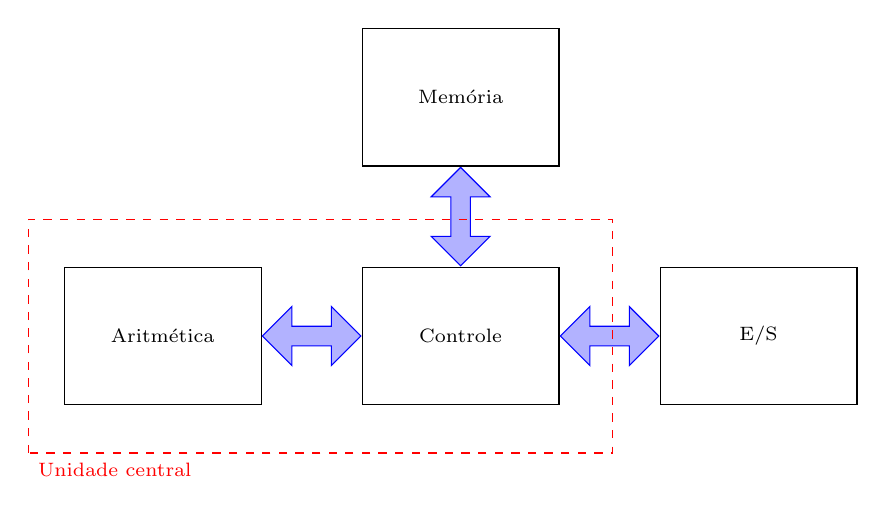
\begin{tikzpicture}[scale=0.9,
  module/.style={anchor=west,draw,rectangle,minimum width=\width,minimum height=\height},
  vdarrow/.style={anchor=west,double arrow,draw=blue,fill=blue!30,minimum height=1.25cm}, % vertical double arrow
  hdarrow/.style={vdarrow,rotate=90} % horizontal double arrow
  ]
  \node[name=a,module] at (0,0) {Aritm\'etica};
  \node[name=ac,vdarrow,shift=(a.east)] {};
  \node[name=c,module,shift=(ac.east)] {Controle};
  \node[name=ces,vdarrow,shift=(c.east)] {};
  \node[name=es,module,shift=(ces.east)] (es) at (2*\height+2*\width,0) {E/S};
  % ATENTION HERE: rotating the double arrow dont change
  % the position names, so east continues being the extremity
  \node[name=ces,hdarrow,shift=(c.north)] {};
  \node[name=mem,module,anchor=south,shift=(ces.east)] {Mem\'oria};
  \draw[dashed,draw=red] (-0.5,-1.65) node[below right]
  {\color{red}{\scriptsize{Unidade central}}} rectangle (7.75,1.65);
\end{tikzpicture}

%\end{frame}

\def\side{3cm}
\def\flabel#1{\scriptsize{#1}}
\begin{frame}
  \frametitle{Organização de um computador simples\footnote{\tiny Figura adaptada de Tanenbaum,2007, pg 29.}}

  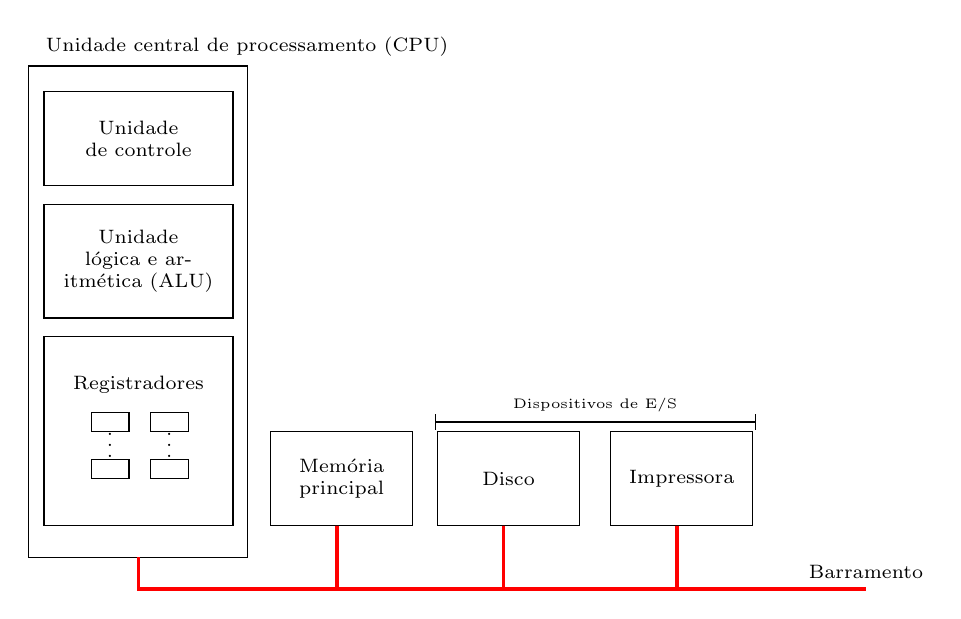
\begin{tikzpicture}[scale=0.8,
    boxtext/.style={text width=2cm,text centered, midway}
    ]
    %CPU
    \draw (0,0) rectangle +(\side,\side);
    \foreach \x / \y in {1/1,2.25/1,1/2,2.25/2} {
      \def\factor{0.25*\side}
      \draw (\factor*\x,\factor*\y) rectangle +(0.2*\side,0.1*\side);
      % draw vertical dots
      \ifnum\y=1%
      \node at (\factor*\x+0.1*\side,\factor*\y+0.22*\side) {$\vdots$};
      \fi
    }
    \node at (0.5*\side,0.75*\side) {\flabel{Registradores}};
    \draw (0,1.1*\side) rectangle +(\side,0.6*\side) 
    node[boxtext] {\flabel{Unidade l\'ogica e aritm\'etica (ALU)}};
    \draw (0,1.8*\side) rectangle +(\side,0.5*\side) 
    node[boxtext] {\flabel{Unidade de controle}};
    % cpu
    \draw (-0.25cm,-0.5cm) rectangle +(0.475cm+\side,2.6*\side)
    node[above] {\flabel{Unidade central de processamento (CPU)}};

    % dev
    \draw (1.2*\side,0) rectangle +(0.75*\side,0.5*\side) 
    node[boxtext] {\flabel{Mem\'oria principal}};
    
    % I/O
    \draw (0.25cm+2*\side,0) rectangle +(0.75*\side,0.5*\side) 
    node[boxtext] {\flabel{Disco}};
    \draw (3*\side,0) rectangle +(0.75*\side,0.5*\side) 
    node[boxtext] {\flabel{Impressora}};
    % I/O label
    \draw[|-|] (0.2cm+2*\side,0.55*\side) -- +(1.7*\side,0) 
    node[midway,above] {{\tiny Dispositivos de E/S}};


    % bus startx at cpu box
    \draw[draw=red,very thick] (0.5*\side,-0.5cm) to (0.5*\side,-1cm)
    to (1.55*\side,-1cm) to (1.55*\side,0)
    to (1.55*\side,-1cm) to (0.25cm+2.35*\side,-1cm)
    to (0.25cm+2.35*\side,0) to (0.25cm+2.35*\side,-1cm)
    to (3.35*\side,-1cm) to (3.35*\side,0)
    to (3.35*\side,-1cm) to (4.35*\side,-1cm) node[above] {\flabel{Barramento}};

    %% becomes noise
    %%\node[text width=3cm] at (4*\side,1.75*\side) {\flabel{1 CPU + 2 dispositivos de entrada e saída}};
  \end{tikzpicture}
  
\end{frame}



%\lecture{Projeto Abstrato}
\subsection{O Processador}
\frame{\Large\bf O Processador}

\begin{frame}{Tarefas de um processador}
  
  Principais tarefas de um processador MIPS divididas por estágios.

  \begin{description}
  \item[\em Instruction fetch stage -- IF $\rightarrow$] Recuperar as
    instruções da memória. \pause
  \item[\em Instruction decode/register file read stage -- ID $\rightarrow$] Ler os
    registradores enquanto decodifica a instrução.\pause
  \item[\em Execution stage -- EX $\rightarrow$] Execução da
    instrução ou cálculo de um endereço.\pause
      \item[\em Memory access stage -- MEM $\rightarrow$] Acessar um
        operando na memória de dados.\pause
      \item[\em Write back stage -- WB $\rightarrow$] Escreve o
        resultado no registrador. 
  \end{description}

\end{frame}


\begin{frame}
\frametitle{Primeiro est\'agio da via de dados}
\vspace{-0.5cm}
{\scriptsize Via de dados de busca de instru\c{c}\~oes e incremento do
  ``contador de programa''(PC)}

\bigskip
\begin{tikzpicture}
  \draw (-1.5,1.5) rectangle ++(1,3) node[midway] {PC};
  \draw[->] (-0.5,3) -- ++(2,0) node[right,text width=2cm]
  {\scriptsize{Endere\c{c}o} lido};
  \draw (1.5,0.2) node[above right] {\tiny \bf mem\'oria de instru\c{c}\~oes}rectangle ++(3,3);
  \node[anchor=east] (instr) at (4.5,1.6) {\scriptsize{Instru\c{c}\~ao}};
  \draw[->] (instr) -- +(2,0);
  \node[draw,trapezium,rotate=-90,minimum height=1.2cm,minimum
  width=1cm] (trap) at (6,4.5) {};
  \draw (trap)+(-0.6cm,0.6cm) -- +(-0.275,0) node[right] {add} -- +(-0.6cm,-0.6cm);
  \draw[draw=white] (trap)+(-0.6cm,0.6cm) -- +(-0.6cm,-0.6cm);
  \draw[<-] (trap)+(-0.6cm,-0.8cm) -- ++(-2cm,-0.8cm) node[left] {4};

  \draw[->] (0.5,3) -- +(0,2.5cm) -- +(4.9,2.5cm);
  \draw[->] (trap.north) -- +(1,0) -- +(1,2) -- +(-9,2) -- +(-9,-1.5)
  -- +(-8.1,-1.5);
\end{tikzpicture}

\end{frame}


% \begin{frame}{Visão abstrata de um processador MIPS}
% \begin{center}
%    \includegraphics[scale=.35]{\imgdir/proc-mips_subset.png}
%   \end{center}
% \end{frame}


\begin{frame}{Processador MIPS32 M4K Core}
{\tiny
  \begin{tabbing}
    \noindent \hspace{1cm}\=FMT -- Fixed mapping translation \hspace{.75cm}\=  MDU -- Integer multiply/divide unit\\
    \noindent \>CP -- CoProcessor \>  \noindent MMU - memory management unit\\
    \noindent \>SRAM -- Static RAM\\
\end{tabbing}
}
\vspace{-1cm}
  \includegraphics[scale=.225]{\imgdir/M4KcoreBlockDiagram.png}

  \vfill
  {\tiny\rm Fonte: MIPS Technologies, Inc. Reproduzida com permissão.}

  \end{frame}


\begin{frame}{Processador MIPS}
  \includegraphics[scale=.25]{\imgdir/M4KcoreBlockDiagram.png}
\end{frame}



\begin{frame}{Outros componentes}

  \begin{description}

  \item[{\em Clock}:] pulso uniforme e com frequência fixa que permite a
    sincronização dos eventos;
  \item[{\em Flip-flop}:] circuito com $2$ estados estáveis usado para
    armazenar informações de estado;
  \item[{\em Latch}:] célula de memória estática;
  \item[Temporizador:] tipo especializado de {\em clock};
  \item[Deslocadores:] deslocamento de bits;
  \item[Registradores] memória do processador.
  \end{description}
  
\end{frame}


\def\thetitle{Arquiteturas: RISC x CISC}
\section{\thetitle}
\frame{\author{}\date{}\institute{}\title{\thetitle}\titlepage}

\begin{frame}{RISC}{Reduced Instruction Set Computer}
  Características
  \begin{itemize}
  \item Conjunto pequeno e simples de instruções;
  \item Instruções executadas no hardware, não havendo microprogramação;
  \item As instruções levam aproximadamente a mesma quantidade de
    tempo para serem executadas;
  \item Maior número de registradores para reduzir o número de acessos
    à memória principal.
  \end{itemize}
  
\end{frame}

\begin{frame}{CISC}{Complex Instruction Set Computer}
  Características:

  \begin{itemize}
  \item Possui um conjunto grande e complexo de instruções, algumas
    armazenadas como código de baixo nível no processador, que fornece
    ao programador de linguagem de montagem uma camada adicional
    chamada microprogramação.
  \end{itemize}

\pause

Vantagens e desvantagens com relação à RISC:

\begin{itemize}
\item Uma vantagem seria fornecer ao programador um número maior de
  operações que na arquitetura RISC deveriam ser codificadas;
\item O outro lado da moeda é que algumas otimizações não podem ser
  feitas na arquitetura CISC devido à impossibilidade de alterar a
  instrução composta com o objetivo de melhorar o desempenho.
\end{itemize}

\end{frame}

\begin{frame}{Leitura Adicional}

\begin{thebibliography}{3}
  \bibitem{tanenbaum2007} [Tanenbaum, 2007]
    {Andrew S. Tanenbaum},
  \newblock {Organização Estruturada de Computadores},
  \newblock {Editora LTC, 2007},

\bibitem{stallings2006}[Stallings, 2006]
  {William Stallings},
  \newblock {Arquitetura e Organização de Computadores},
  \newblock {Makron Books, 2006}

\bibitem{patterson2008}[Patterson, 2008]
  {David A. Patterson; John L. Hennessy},
  \newblock                {Computer Organization and Design},
  \newblock    {Morgan Kaufmann Publisher, 2008},

\end{thebibliography}

\end{frame}

\end{document}


%%%%%%%%%%%%%%%%%%%%%%%%%%%%%%%%%%%%%%%%%%%%%%%%%%%%%%%%%%%%%%%%%%%%%
%                                BUFFER
%%%%%%%%%%%%%%%%%%%%%%%%%%%%%%%%%%%%%%%%%%%%%%%%%%%%%%%%%%%%%%%%%%%%%



\def\bit#1{{\tt #1}}
\def\comment#1{{\tiny #1}}
\def\linelabel#1{{\tiny #1}}

\def\reg{\only<2>{\color{red}}\only<3->{\color{gray}}}
\def\immed{\only<3>{\color{red}}\only<2,4->{\color{gray}}}
\def\jump{\only<4>{\color{red}}\only<2,3,5->{\color{gray}}}

\begin{frame}
  \frametitle{Instru\c{c}\~oes MIPS} 

% pg 128
  
\begin{scriptsize}
\begin{tabular}[ht]{|l|c|c|c|c|c|c|l|}\hline
  \multicolumn{1}{|c|}{Nome} & \multicolumn{6}{|c|}{Campos} & \multicolumn{1}{|c|}{Descri\c{c}\~ao} \\ \hline
  
  \linelabel{Tamanho} &\bit{6} & \bit{5} & \bit{5} & \bit{5} & \bit{5} & \bit{6} &
  \comment{Todas as intru\c{c}\~oes MIPS s\~ao de 32 bits} \\ \hline
  
  \reg \linelabel{Formato-\bf{R}} & \reg op & \reg rs & \reg rt & \reg
  rd & \reg \tt{shamt} & \reg funct & \reg
  \comment{Formato de instru\c{c}\~ao aritm\'etica} \\ \hline

  \immed \linelabel{Formato-\bf{I}} & \immed op & \immed rs & \immed
  rt &  \multicolumn{3}{|c|}{\immed endere\c{c}o/imediato} &
  \immed \comment{Formato de transferência, desvio e constante} \\ \hline
  
  \jump \linelabel{Formato-\bf{J}} & \jump op & \multicolumn{5}{|c|}{\jump endere\c{c}o} &
  \jump \comment{Formato de instru\c{c}\~{a}o {\em jump}} \\ \hline
\end{tabular}


\only<1>{
\vspace{0.64cm}
% pg 100
\begin{tabular}[ht]{|l|c|c|c|c|c|c|c|l|}\hline

  \multicolumn{1}{|c|}{Nome} & Formato & \multicolumn{6}{|c|}{Exemplo} & \multicolumn{1}{|c|}{Descri\c{c}\~ao} \\ \hline
  
  add & R & 0 & 18 & 19 & 17 & 0 & 32 & add \tt{\$s1,\$s2,\$s3} \\
  \hline

  sub & R & 0 & 18 & 19 & 17 & 0 & 34 & sub \tt{\$s1,\$s2,\$s3} \\
  \hline

    addi & I & 35 & 18 & 17 & \multicolumn{3}{|c|}{100} &  addi
    \tt{\$s1,\$s2,100} \\ \hline
    
    lw & I & 43 & 18 & 17 & \multicolumn{3}{|c|}{100} &  lw
    \tt{\$s1,\$s2,100(\$s2)} \\ \hline

    sw & I & 8 & 18 & 17 & \multicolumn{3}{|c|}{100} &  sw
    \tt{\$s1,\$s2,100(\$s2)} \\ \hline

   % jr & I & 31 & \multicolumn{5}{|c|}{31} &  jr \tt{\$ra} \\ \hline

\end{tabular}
} % only 1

\only<2->{
\begin{block}{\alert<2>{Instru\c{c}\~oes reg-reg (op == 0)}}
  \only<2>{
  \begin{tabular}[ht]{ll}
      -- add, sub, and, or, nor, xor, slt & \texttt{R[rd] $\leftarrow$
        R[rs] funct R[rt]; \hfill PC $\leftarrow$ PC + 4;} \\
      -- sll, srl, sra & \texttt{R[rd] $\leftarrow$ R[rt] shift shamt;} \\
    \end{tabular}
  }
\end{block}
}

\only<3->{
\begin{block}{\alert<3>{Instru\c{c}\~oes reg-const (op != 0)}}
  \only<3>{
  \begin{tabular}[ht]{ll}
    -- addi, andi, ori, xori  & \texttt{R[rd] $\leftarrow$
      R[rs] op lm 16}; \\
      -- lui, addiu, slti, sltiu & \\
      -- lw, lh, lhu, lb, lbu & \texttt{R[rt] $\leftarrow$ Mem[ R[rs]
        + signEx(lm 16) ];} \\
      -- sw, sh, sb & \texttt{Mem[R[rs] + signEx(lm 16)]
        $\leftarrow$ R[rt];} \\
    \end{tabular}
  }
\end{block}
}


\only<4->{
\begin{block}{\alert<4>{\em Jumps}}
  \only<4>{
  \begin{tabular}[ht]{ll}
    -- j  & \texttt{PC $\leftarrow$ PC$_{31,28}$ || endere\c{c}o || 00;} \\
      -- jal & \texttt{PC $\leftarrow$ PC$_{31,28}$ || endere\c{c}o ||
        00; \hfill R[31] $\leftarrow$ PC + 4;} \\
      -- jr & \texttt{PC $\leftarrow$ R[rs];} \\
    \end{tabular}
  }
\end{block}
}

\only<5->{
\begin{block}{\alert<4>{Desvios}}
  \only<5>{
  \begin{tabular}[ht]{ll}
    -- beq, ben  & \texttt{PC $\leftarrow$ (R[rs] ?= R[rt]) ? PC +
      signEx(lm 16) : PC + 4;} \\
      -- blt, bgt, ble, bgte & \texttt{pseudo instru\c{c}\~oes} \\
    \end{tabular}
  }
\end{block}
}



\end{scriptsize}


\end{frame}






\lecture{Componentes}

\section{\insertlecture}

\frame{\Large\bf \insertlecture}

\begin{frame}[fragile]{Multiplexador}

Para $2^n$ linhas de entrada o \alert{multiplexador} seleciona $n$ saídas.\\

Exemplo:

\begin{columns}
\begin{column}{.4\textwidth}

 \begin{center}
   
\includegraphics[scale=0.4]{../fig/proc-multiplexer.png}
 \end{center}

\end{column}

\begin{column}{.6\textwidth}

\begin{tikzpicture}[use US style logic gates,
tiny circuit symbols,
allgate/.style={minimum width=1.5cm,draw}]

\node [and gate,allgate, logic gate inputs=ni] (a1) {};
\node (A) [left of=a1,xshift=-10mm,yshift=2mm] {A};
\node [or gate,draw,allgate] (o) [right of=a1,xshift=15mm,
yshift=-5mm] {}; \node (C) [right of=o,xshift=10mm] {C};
\node [and gate,draw, allgate, logic gate inputs=nn] (a2)
[below of=a1, yshift=-5mm] {};
\node (B) [left of=a2,xshift=-10mm, yshift=-2mm] {B};
\node (S) [below of=a2,xshift=-17.5mm] {S};

\draw (A)  -- (a1.input 1);
\draw (S.east) -- ++(right:3mm) |-  (a1.input 2);
\draw (S.east) -- ++(right:3mm) |- (a2.input 1);
\draw (B.east) --  (a2.input 2);
\draw (a1.output) -- ++(right:3mm) |- (o.input 1);
\draw (a2.output) -- ++(right:3mm) |- (o.input 2);
\draw (o.output)  -- (C);

\end{tikzpicture}
\end{column}  
\end{columns}

\begin{equation}
 \label{eq:mux}
 C = (A\cdot\overline{S})+(B\cdot S)
\end{equation}

\end{frame}

\begin{frame}[fragile]{Decodificador}

Para $n$ linhas de entrada o \alert{decodificador} gera $2^n$ saídas.\\

Exemplo:

 \begin{center}
   \includegraphics[scale=0.4]{../fig/proc-decoder.png}
 \end{center}
\end{frame}

\begin{frame}[fragile]{Multiplexador -- exemplo de uso}
 \begin{center}
   \includegraphics[scale=0.4]{../fig/proc-mux_example.png}
 \end{center}
\end{frame}

\begin{frame}{\em Clock}

  \begin{itemize}
  \item<1> Elementos e operações em um ciclo de clock.
  \item<2> Redução de um elemento de estado devido à escrita ser
    realizado na borda ascendente do {\bf clock}.
  \end{itemize}
  
  \begin{center}
    \includegraphics<1>[scale=.5]{../fig/proc-clock_cycle1.png}
    
    \includegraphics<2>[scale=.5]{../fig/proc-clock_cycle2.png}
  \end{center}

\end{frame}


\end{frame}
%%% Local Variables:
%%% TeX-master: main
%%% End:

\lecture{O Processador}{theproc}

 \lecturetitle{\insertlecture}{\course}

 \frame{\maketitle}
 \part{\insertlecture}
 \frame{\frametitle{Trilha}\tableofcontents}

 \section{Introdução}

\framefigtanenbaum{}


\framemipsprocfigure{}


 \begin{frame}{Tarefas de um processador}

   Principais tarefas de um processador MIPS divididas por estágios.

   \begin{description}
   \item[\em Instruction fetch stage -- IF $\rightarrow$] Recuperar as
     intruções da memória. \pause
   \item[\em Instruction decode/register file read stage -- ID $\rightarrow$] Ler os
     registradores enquanto decodifica a instrução.\pause
   \item[\em Execution stage -- EX $\rightarrow$] Execução da
     instrução ou cálculo de um endereço.\pause
       \item[\em Memory access stage -- MEM $\rightarrow$] Acessar um
         operando na memória de dados.\pause
       \item[\em Write back stage -- WB $\rightarrow$] Escreve o
         resultado no registrador. 
   \end{description}

 \end{frame}

\def\thetitle{Componentes}

\section{\thetitle}

\frame{\author{}\date{}\institute{}\title{\thetitle}\titlepage}

\begin{frame}[fragile]{Multiplexador}

Para $2^n$ linhas de entrada o \alert{multiplexador} seleciona $n$ saídas.\\

Exemplo:

\begin{columns}
\begin{column}{.4\textwidth}

  \begin{center}
%    
\includegraphics[scale=0.4]{\imgdir/proc-multiplexer.png}
  \end{center}

\end{column}

\begin{column}{.6\textwidth}

\begin{tikzpicture}[use US style logic gates,
%tiny circuit symbols,
allgate/.style={minimum width=1.5cm,draw}]

\node [and gate,allgate, logic gate inputs=ni] (a1) {};
\node (A) [left of=a1,xshift=-10mm,yshift=2mm] {A};
\node [or gate,draw,allgate] (o) [right of=a1,xshift=15mm,
yshift=-5mm] {}; \node (C) [right of=o,xshift=10mm] {C};
\node [and gate,draw, allgate, logic gate inputs=nn] (a2)
[below of=a1, yshift=-5mm] {};
\node (B) [left of=a2,xshift=-10mm, yshift=-2mm] {B};
\node (S) [below of=a2,xshift=-17.5mm] {S};

\draw (A)  -- (a1.input 1);
\draw (S.east) -- ++(right:3mm) |-  (a1.input 2);
\draw (S.east) -- ++(right:3mm) |- (a2.input 1);
\draw (B.east) --  (a2.input 2);
\draw (a1.output) -- ++(right:3mm) |- (o.input 1);
\draw (a2.output) -- ++(right:3mm) |- (o.input 2);
\draw (o.output)  -- (C);

\end{tikzpicture}
\end{column}  
\end{columns}

\begin{equation}
  \label{eq:mux}
  C = (A\cdot\overline{S})+(B\cdot S)
\end{equation}

\end{frame}

\begin{frame}[fragile]{Decodificador}

Para $n$ linhas de entrada o \alert{decodificador} gera $2^n$ saídas.\\

Exemplo:

  \begin{center}
    \includegraphics[scale=0.4]{proc-decoder.png}
  \end{center}
\end{frame}

\begin{frame}[fragile]{Multiplexador -- exemplo de uso}
  \begin{center}
    \includegraphics[scale=0.4]{proc-mux_example.png}
  \end{center}
\end{frame}

\begin{frame}{\em Clock}

  \begin{itemize}
  \item<1> Elementos e operações em um ciclo de clock.
  \item<2> Redução de um elemento de estado devido à escrita ser
    realizado na borda ascendente do {\bf clock}.
  \end{itemize}
  
  \begin{center}
    \includegraphics<1>[scale=.5]{proc-clock_cycle1.png}
    
    \includegraphics<2>[scale=.5]{proc-clock_cycle2.png}
  \end{center}

\end{frame}

\begin{frame}{Outros componentes}

  \begin{itemize}
  \item {\em Flip-flop}: circuito com $2$ estados estáveis usado para
    armazenar informações de estado;
  \item {\em Latch}: célula de memória estática;
  \item Temporizador: tipo especializado de {\em clock};
  \item Deslocadores;
  \item Registradores: memória do processador.
  \end{itemize}
  
\end{frame}


\def\thetitle{Projeto abstrato}
\frame{\author{}\date{}\institute{}\title{\thetitle}\titlepage}

\section{\thetitle}

\begin{frame}
\frametitle{Primeiro est\'agio da via de dados}
\vspace{-0.5cm}
{\scriptsize Via de dados de busca de instru\c{c}\~oes e incremento do
  ``contador de programa''(PC)}

\bigskip
\begin{tikzpicture}
  \draw (-1.5,1.5) rectangle ++(1,3) node[midway] {PC};
  \draw[->] (-0.5,3) -- ++(2,0) node[right,text width=2cm]
  {\scriptsize{Endere\c{c}o} lido};
  \draw (1.5,0.2) node[above right] {\tiny \bf mem\'oria de instru\c{c}\~oes}rectangle ++(3,3);
  \node[anchor=east] (instr) at (4.5,1.6) {\scriptsize{Instru\c{c}\~ao}};
  \draw[->] (instr) -- +(2,0);
  \node[draw,trapezium,rotate=-90,minimum height=1.2cm,minimum
  width=1cm] (trap) at (6,4.5) {};
  \draw (trap)+(-0.6cm,0.6cm) -- +(-0.275,0) node[right] {add} -- +(-0.6cm,-0.6cm);
  \draw[draw=white] (trap)+(-0.6cm,0.6cm) -- +(-0.6cm,-0.6cm);
  \draw[<-] (trap)+(-0.6cm,-0.8cm) -- ++(-2cm,-0.8cm) node[left] {4};

  \draw[->] (0.5,3) -- +(0,2.5cm) -- +(4.9,2.5cm);
  \draw[->] (trap.north) -- +(1,0) -- +(1,2) -- +(-9,2) -- +(-9,-1.5)
  -- +(-8.1,-1.5);
\end{tikzpicture}

\end{frame}

\begin{frame}{Visão abstrata de um processador MIPS}
\begin{center}
    \includegraphics[scale=.35]{proc-mips_subset.png}
  \end{center}
\end{frame}


\def\thetitle{Arquiteturas: RISC x CISC}
\section{\thetitle}
\frame{\author{}\date{}\institute{}\title{\thetitle}\titlepage}

\begin{frame}{RISC}{Reduced Instruction Set Computer}
  Características
  \begin{itemize}
  \item Conjunto pequeno e simples de instruções;
  \item Instruções executadas no hardware, não havendo microprogramação;
  \item As instruções levam aproximadamente a mesma quantidade de
    tempo para serem executadas;
  \item Maior número de registradores para reduzir o número de acessos
    à memória principal.
  \end{itemize}
  
\end{frame}

\begin{frame}{CISC}{Complex Instruction Set Computer}
  Características:

  \begin{itemize}
  \item Possui um conjunto grande e complexo de instruções, algumas
    armazenadas como código de baixo nível no processador, que fornece
    ao programador de linguagem de montagem uma camada adicional
    chamada microprogramação.
  \end{itemize}

\pause

Vantagens e desvantagens com relação à RISC:

\begin{itemize}
\item Uma vantagem seria fornecer ao programador um número maior de
  operações que na arquitetura RISC deveriam ser codificadas;
\item O outro lado da moeda é que algumas otimizações não podem ser
  feitas na arquitetura CISC devido à impossibilidade de alterar a
  instrução composta com o objetivo de melhorar o desempenho.
\end{itemize}

\end{frame}

\begin{frame}{Referência}
  
  \begin{columns}
    \begin{column}{0.3\textwidth}
      
\includegraphics[scale=2]{\imgdir/patterson-book_cover.png}

    \end{column}
    \begin{column}{0.7\textwidth}
\small
      Computer Organization and Design, 4th Edition\\
      The Hardware/Software Interface.\\
      David A. Patterson  \&  John L. Hennessy \\
      Morgan Kaufmann Publisher\\
      ISBN: 978-0-12-374493-7\\
      2008
    \end{column}
  \end{columns}

\end{frame}

\end{document}

\lecture{Portas Lógicas}{Unidades básicas}

\subsection{\insertlecture}

\begin{frame}[fragile]{Portas Lógicas}
\def\shift{2cm}
\tikzset{every node/.style={font=\scriptsize}}

\begin{circuitikz}
\draw (0,0) node[and port] (AND) {};
\node [above of=AND,xshift=-.45*\shift] {\tt AND};
\node [below of=AND,xshift=-.45*\shift] {\tt $S=A.B$};

\draw (1.5*\shift,0) node[or port] (OR) {};
\node [above of=OR,xshift=-.45*\shift] {\tt OR};
\node [below of=OR,xshift=-.45*\shift] {\tt $S=A+B$};

\draw (2.5*\shift,0) node[not port] (NOT) {};
\node [above of=NOT,xshift=-.15*\shift] {\tt NOT};
\node [below of=NOT,xshift=-.15*\shift] {\tt $S=\NOT{A}$};

\draw (4*\shift,0) node[xor port] (XOR) {};
\node [above of=XOR,xshift=-.45*\shift] {\tt XOR};
\node [below of=XOR,xshift=-.45*\shift] {\tt $S=A\bigoplus B$};

\foreach \G in {AND, OR, XOR} {
  \node[above] at (\G.in 1) {A};
  \node[below] at (\G.in 2) {B};
  \node[above] at (\G.out) {\color{out}S};
}
  \node[above] at (NOT.in) {A};
  \node[above] at (NOT.out) {\color{out}S};

\matrix [below of=AND,yshift=-\shift,xshift=-.35*\shift] (and table){
  \A & \B & \color{out} \S \\\hline
  \O & \O & \color{out}\O\\
  \O & \I & \color{out}\O\\
  \I & \O & \color{out}\O\\
  \I & \I & \color{out}\I\\
};

\matrix [below of=OR,yshift=-\shift,xshift=-.35*\shift] (and table){
  \A & \B & \color{out}\S \\\hline
  \O & \O & \color{out}\O\\
  \O & \I & \color{out}\I\\
  \I & \O & \color{out}\I\\
  \I & \I & \color{out}\I\\
};

\matrix [below of=NOT,yshift=-.75*\shift,xshift=-.15*\shift] (and table){
  \A & \color{out}\S \\\hline
  \O & \color{out}\I\\
  \I & \color{out}\O\\
};

\matrix [below of=XOR,yshift=-\shift,xshift=-.35*\shift] (and table){
  \A & \B & \color{out}\S \\\hline
  \O & \O & \color{out}\O\\
  \O & \I & \color{out}\I\\
  \I & \O & \color{out}\I\\
  \I & \I & \color{out}\O\\
};


\end{circuitikz}

\end{frame}

\subsection{Controle}

\frame{\centering{\bf\large Controle}}

\begin{frame}{Decodificador}

Para \alert{$k$} entradas, o \alert{decodificador} seleciona entre \alert{$2^k$} saídas.

\begin{center}
 
%%% Local Variables:
%%% mode: latex
%%% TeX-master: t
%%% End:
\begin{tikzpicture}

\def\shift{2cm}

\tikzset{
    every node/.style={font=\scriptsize}, 
    wire/.style={->, >=latex, draw},
    decoder/.style={minimum width=\shift,minimum height=\shift,draw},
    header/.style={minimum width=1.5*\shift,white},
    in header/.style={header, fill=green!65!black},
    out header/.style={header, fill=red!80!black}
}

\node[decoder] (DECODER) at (0,0) {decodificador};
\node (out tip) at (\shift, 0) {};
\node (in tip) at (-\shift, 0) {};

\newcounter{lout}\setcounter{lout}{0}
\foreach \i in {-4,-3,-2,-1,0,1,2,3} {
    \path[wire] (.5*\shift,.225*\i+.1) -- (\shift,.225*\i+.1) node[right]{\tiny \arabic{lout}};
    \addtocounter{lout}{1}
}

\path[wire] (in tip) node[above right] {\tiny 3} -- (DECODER);
\path[draw] (in tip.south east)+(.2*\shift,0) -- +(.08*\shift,.2*\shift);

\matrix [right of=DECODER, xshift=2.5*\shift] (truth table) {
    \node[in header]{Entradas};&\node[out header]{Sa\'idas};\\     
    \node[in header]{2\ \ 1\ \ 0};&\node[out header]{7\ \ 6\ \ 5\ \ 4\ \ 3\ \ 2\ \ 1\ \ 0};\\     
    \node{0\ \ 0\ \ 0}; & \node{0\ \ 0\ \ 0\ \ 0\ \ 0\ \ 0\ \ 0\ \ 1};\\
    \node{0\ \ 0\ \ 1}; & \node{0\ \ 0\ \ 0\ \ 0\ \ 0\ \ 0\ \ 1\ \ 0};\\
    \node{0\ \ 1\ \ 0}; & \node{0\ \ 0\ \ 0\ \ 0\ \ 0\ \ 1\ \ 0\ \ 0};\\
    \node{0\ \ 1\ \ 1}; & \node{0\ \ 0\ \ 0\ \ 0\ \ 1\ \ 0\ \ 0\ \ 0};\\
    \node{1\ \ 0\ \ 0}; & \node{0\ \ 0\ \ 0\ \ 1\ \ 0\ \ 0\ \ 0\ \ 0};\\
    \node{1\ \ 0\ \ 1}; & \node{0\ \ 0\ \ 1\ \ 0\ \ 0\ \ 0\ \ 0\ \ 0};\\
    \node{1\ \ 1\ \ 0}; & \node{0\ \ 1\ \ 0\ \ 0\ \ 0\ \ 0\ \ 0\ \ 0};\\
    \node{1\ \ 1\ \ 1}; & \node{1\ \ 0\ \ 0\ \ 0\ \ 0\ \ 0\ \ 0\ \ 0};\\
};

\node [above of=truth table, yshift=\shift] {Tabela-Verdade};
\end{tikzpicture}

                    
\end{center}

\end{frame}
    
\begin{tikzpicture}
  
\def\shift{1cm}
\begin{scope}
  \tikzset{every node/.style={font=\scriptsize},
   every path/.style={->,>=latex, draw},
    mux/.style={rotate=90, minimum height=.5*\shift,minimum width=2*\shift, rounded
      corners=2mm, draw},
    l/.style={gray}
}

    \node[mux] (MUX) at (0,0) {};
    \node[l] (M) at ([yshift=.25*\shift]MUX) {m};
    \node[l] (u) [below of=M,yshift=.75\shift] {u};
    \node[l] (x) [below of=u,yshift=.75\shift] {x};

    \node at ([xshift=-1.5*\shift]MUX.20) (A) {x};
  
    \path  (A) -- (MUX.20) node[right,xshift=1] {$0$};

    \node (B) at ([xshift=-1.5*\shift]MUX.160) {y};
  
    \path (B) -- (MUX.160) node[right,xshift=1] {$1$};

    \node (C) at ([xshift=1.5*\shift]MUX.south) {f};
  
    \path  (MUX.south) -> (C);
  
    \node (S) at ([yshift=-1.5*\shift]MUX.west) {seleção $s$};
  
    \path[->,>=latex]  (S) -> (MUX.west);

    

   \matrix (select table) [matrix of nodes, above of=MUX,xshift=-.5\shift,yshift=\shift]
   {
     \bf s & \bf f \\
     0 & =x \\
     1 & =y \\
   };

\end{scope}

\begin{scope}

  %GATES
  \draw
  (5,1) node[and gate US,draw] (andA){}
  (5,-1) node[and gate US,draw] (andB){}
  (7,0) node[or gate US,draw] (orC){}
  (andA.output) -| (orC.input 1)
  (andB.output) -| (orC.input 2);
  \node[above] (LC) at (orC.output) {$f$};

  %+WIRE
  \path[draw] (andA.input 1) node[] (anchor A) {} -- +(-.5,0) node[above] {x};
  \path[draw] (andB.input 2) node[] (anchor B) {} -- +(-.5,0) node[above] {y};

  \node[] at (andA.input 2) (wire inAtwo)  {};
  \node[ocirc] [right of=wire inAtwo,xshift=-.8*\shift] {};

  % SIGNAL
  \node[right] (S) [below of=anchor B] {seleção $s$};
  \path[draw] (S) -- (andB.input 1) node[circ] {} -- (andA.input 2);

   \node[green!30!black] (EXP) [below of=orC,xshift=.125*\shift,yshift=-\shift] {$f~(s,x,y) = x\overline{s} + ys$};
   

  \end{scope}
  
\end{tikzpicture}


\subsection{Lógica}
\frame{\centering{\bf\large Lógica}}

\begin{frame}
\frametitle{Unidade Lógica de 1-bit}

\begin{center}
\def\NOT#1{\overline{#1}}

\begin{circuitikz}
\def\shift{2cm}

\colorlet{aincolor}{green!45!black}
\colorlet{bincolor}{blue!45!black}
\colorlet{outcolor}{red!80!black}

\tikzset{
    every path/.style={draw},
    every node/.style={font=\scriptsize}, 
    wire/.style={->, >=latex, draw},
    header/.style={minimum width=1.*\shift,white},
    a header/.style={header, fill=aincolor},
    b header/.style={header, fill=bincolor},
    out header/.style={header, fill=outcolor},
    mux/.style={ minimum height=.2*\shift,minimum width=2.5*\shift, rotate=90,
      rounded corners=2mm, draw}
}

%GATES
\draw (0,1.475) node[or port] (OR) {};
\draw (0,-1.475) node[and port] (AND) {};

%WIRES
\path[aincolor]  (OR.in 1) -- +(-1,0) node[above] (A) {$A$};
\path[bincolor]   (AND.in 2) -- +(-1,0) node[above] (B) {$B$};
\path[aincolor]  (A.south east) node[circ] {} -- +(0,-2.95) |- (AND.in 1);
\path[bincolor]  (B.south east)+(.78,0) node[circ] {} -- +(.75,2) |- (OR.in 2);

\node[mux] (MUX) at (1,0) {\color{gray}mux};
\node (zero) at ([yshift=.75*\shift]MUX) {$0$};
\node (one) [below of=zero,yshift=-.95*\shift] {$1$};


\path[wire] (OR.out) -- (MUX.8);
\path[wire] (AND.out) -- (MUX.172);
\path[wire] (MUX.south) -- +(\shift,0) node (C) [above] {$C$};
\path[<-,>=latex,red] (MUX.west) node[below right] {$S$} -- +(0,-.5*\shift);


\node [below of=C,xshift=.75*\shift] {$C=(A+B){\color{red}\NOT{S}} + (A.B).{\color{red}S}$};

\end{circuitikz}

\end{center}

\end{frame}


\subsection{Aritmética}

\frame{\centering{\bf\large Aritmética}}

\begin{frame}
\frametitle{Somador Parcial}

\begin{center}
\begin{circuitikz}
\def\shift{2cm}

\colorlet{aincolor}{green!75!black}
\colorlet{bincolor}{green!35!black}
\colorlet{outcolor}{red!80!black}

\tikzset{
    every path/.style={draw},
    every node/.style={font=\scriptsize}, 
    wire/.style={->, >=latex, draw},
    header/.style={minimum width=1.*\shift,white},
    a header/.style={header, fill=aincolor},
    b header/.style={header, fill=bincolor},
    out header/.style={header, fill=outcolor}
}

%GATES
\draw (0,1) node[xor port] (XOR) {};
\draw (0,-1) node[and port] (AND) {};

%WIRES

% PATHS
\path[outcolor] (XOR) -- +(1,0) node[above] {Soma};
\path[outcolor] (AND) -- +(1,0) node[below] {Vai-um};

\path[aincolor]  (XOR.in 1) -- +(-1,0) node[above] (A) {A};
\path[bincolor]   (AND.in 2) -- +(-1,0) node[above] (B) {B};
\path[aincolor]  (A.south east) node[circ] {} -- +(0,-2) -- (AND.in 1);
\path[aincolor]  (B.south east)+(.5,0) node[circ] {} -- +(.5,2) -- (XOR.in 2);

%\path[incolor]  (B) -| (AND.in 2);


\matrix [right of=XOR, xshift=2*\shift,yshift=-.85\shift] (truth table) {
    \node[a header]{Entradas};&\node[out header]{Sa\'idas};\\     
    \node[b header]{A\ \ B};&\node[out header]{Soma\ \ Vai-um};\\     
    \node{0\ \ 0}; & \node{0\ \ \ 0};\\
    \node{0\ \ 1}; & \node{1\ \ \ 0};\\
    \node{1\ \ 0}; & \node{1\ \ \ 0};\\
    \node{1\ \ 1}; & \node{0\ \ \ 1};\\
};

\node [above of=truth table, yshift=.5*\shift] {Tabela-Verdade};

\node [above of=XOR, yshift=.25*\shift] (CARRY) {Vai-um$=A.B$};
\node [above of=CARRY,yshift=-.25*\shift] (SUM) {Soma$=A\bigoplus B$};

\end{circuitikz}

\end{center}

\end{frame}

\begin{frame}{Somador Completo}{Circuito}

\begin{center}
\begin{circuitikz}
\def\shift{2cm}

\colorlet{aincolor}{green!75!black}
\colorlet{bincolor}{blue!35!black}
\colorlet{outcolor}{red!80!black}

\tikzset{
    every path/.style={draw},
    every node/.style={font=\scriptsize}, 
    wire/.style={->, >=latex, draw},
    header/.style={minimum width=1.*\shift,white},
    a header/.style={header, fill=aincolor},
    b header/.style={header, fill=bincolor},
    out header/.style={header, fill=outcolor}
}

%GATES
\draw (0,1.54) node[xor port] (XOR) {};
\draw (2.5,1.25) node[xor port] (XOR SUM) {};

\draw (1.75,0) node[and port] (AND CIN) {};

\draw (3.5,-1.25) node[or port] (COUT) {};
\draw (0,-1.5) node[and port] (AND) {};

%WIRES

% PATHS
\path[outcolor] (XOR SUM.out) -- +(2,0) node[above] {$S$};
\path[outcolor] (COUT.out) -- +(1,0) node[below] {$Vai$-um};

\path[aincolor]  (XOR.in 1) -- +(-1,0) node[above] (A) {$A$};
\path[bincolor]   (AND.in 2) -- +(-1,0) node[above] (B) {$B$};
\path[aincolor]  (A.south east) node[circ] {} -- +(0,-1) |- (AND.in 1);
\path[aincolor]  (B.south east)+(.5,0) node[circ] {} -- +(.5,2) |- (XOR.in 2);

%%CIN
\path[brown!45!black] (AND CIN.in 2) -- +(-2.75,0) node[above] {$Vem$-um};

%%SUM
\path (XOR.out) -- (XOR SUM.in 1);
\path (AND CIN.in 1) |- node[circ] {} (XOR SUM.in 1);

%%COUT
\path (AND CIN.out) -| (COUT.in 1);
\path (AND.out) -- (COUT.in 2);
\path (XOR SUM.in 2) -- +(-1.25,0) |- node[circ] {} (AND CIN.in 2);

\end{circuitikz}

\end{center}

\end{frame}

\begin{frame}{Somador Completo}{Símbolo}

\begin{center}

%%% Local Variables:
%%% mode: latex
%%% TeX-master: t
%%% End:
\begin{circuitikz}
\def\shift{2cm}

\colorlet{aincolor}{green!75!black}
\colorlet{bincolor}{green!35!black}
\colorlet{outcolor}{red!80!black}

\tikzset{
    every path/.style={->, >=latex, draw},
    every node/.style={font=\scriptsize}, 
    wire/.style={->, >=latex, draw},
    adder/.style={minimum width=3cm, minimum height=3cm,draw},
    header/.style={minimum width=1.*\shift,white},
    a header/.style={header, fill=aincolor},
    b header/.style={header, fill=bincolor},
    out header/.style={header, fill=outcolor}
}

\node[adder] (ADDER) {\LARGE $+$};
\path (ADDER.north)+(0,0.5*\shift) node[above] {C$_{in}$} -- (ADDER);
\path (ADDER.south) -- +(0,-0.5*\shift) node[below] {C$_{out}$};
\path (ADDER.east) -- +(0.5*\shift,0) node[below] {S};
\path (ADDER.west)+(-.5*\shift,.25*\shift)  node[above] {A}  -- +(0,.25*\shift);
\path (ADDER.west)+(-.5*\shift,-.25*\shift) node[below] {B} -- +(0,-.25*\shift);

\matrix [right of=ADDER, xshift=2*\shift,yshift=-.25\shift] (truth table) {
    \node[a header]{Entradas};&\node[out header]{Sa\'idas};\\     
    \node[b header]{A\ \ \ \ B\ \ \ C$_{in}$};&\node[out header]{C$_{out}$\ \ \ S};\\     
    \node{0\ \ \ \ 0\ \ \ \ 0}; & \node{0\ \ \ \ \ 0};\\
    \node{0\ \ \ \ 0\ \ \ \ 1}; & \node{0\ \ \ \ \ 1};\\
    \node{0\ \ \ \ 1\ \ \ \ 0}; & \node{0\ \ \ \ \ 1};\\
    \node{0\ \ \ \ 1\ \ \ \ 1}; & \node{1\ \ \ \ \ 0};\\
    \node{1\ \ \ \ 0\ \ \ \ 0}; & \node{0\ \ \ \ \ 1};\\
    \node{1\ \ \ \ 0\ \ \ \ 1}; & \node{1\ \ \ \ \ 0};\\
    \node{1\ \ \ \ 1\ \ \ \ 0}; & \node{1\ \ \ \ \ 0};\\
    \node{1\ \ \ \ 1\ \ \ \ 1}; & \node{1\ \ \ \ \ 1};\\
};

\node [above of=truth table, yshift=\shift] {Tabela-Verdade};

\end{circuitikz}

\end{center}

\end{frame}

\begin{frame}{Somador Completo de 32 bits}

\begin{center}

%%% Local Variables:
%%% mode: latex
%%% TeX-master: t
%%% End:

\begin{circuitikz}
\def\shift{1.5cm}

\colorlet{aincolor}{green!75!black}
\colorlet{bincolor}{green!35!black}
\colorlet{outcolor}{red!80!black}

\tikzset{
    every path/.style={->, >=latex, draw},
    every node/.style={font=\scriptsize}, 
    wire/.style={->, >=latex, draw},
    adder/.style={minimum width=1cm, minimum height=1cm,draw},
}

\foreach \i/\prev/\idx/\cur in {0/0/0/31,1/0/31/3,2/1/2/2,3/2/1/1} {
  \node[adder] at (0,\i*\shift) (adder\i) {\LARGE $+$};
  \node[anchor=west] at (adder\i.150) (a\i) {};
  \node[anchor=west] at (adder\i.210) (b\i) {};
  \node[anchor=east] at (adder\i.east) (s\i) {};
  \path[wire] (a\i)+(-.5*\shift,0) -- (a\i) node[midway,above] {A$_{\cur}$};
  \path[wire] (b\i)+(-.5*\shift,0) -- (b\i) node[midway,above] {B$_{\cur}$};
  \path[wire] (s\i) -- +(.5*\shift,0) node[midway,above] {S$_{\cur}$};
  
  \ifnum\i=0
  {}
  \else\ifnum\idx=31
    \path[wire,dotted,red] (adder\i.south) -- (adder\prev.north) node[midway,right] {C$_{out\idx}$};
  \else
  \path[wire] (adder\i.south) -- (adder\prev.north) node[midway,right] {C$_{out}\idx$};
  \fi\fi
}

\node[adder] at (0,4*\shift) (adder4) {\LARGE $+$};
  \node[anchor=west] at (adder4.150) (a4) {};
  \node[anchor=west] at (adder4.210) (b4) {};
  \node[anchor=east] at (adder4.east) (s4) {};
  \path[wire] (adder4.south) -- (adder3.north) node[midway,right] {C$_{out}0$};
  \path[wire] (a4)+(-.5*\shift,0) -- (a4) node[midway,above] {A$_0$};
  \path[wire] (b4)+(-.5*\shift,0) -- (b4) node[midway,above] {B$_0$};
  \path[wire] (s4) -- +(.5*\shift,0) node[midway,above] {S$_0$};
\end{circuitikz}

\end{center}

\end{frame}



\frame{\centering{\bf\large Unidade Lógica e Aritmética (ULA)}}

\begin{frame}{ULA de 1-bit}{Circuito}

\begin{center}

%%% Local Variables:
%%% mode: latex
%%% TeX-master: t
%%% End:

\begin{circuitikz}
\def\shift{1.5cm}

\colorlet{aincolor}{green!75!black}
\colorlet{bincolor}{blue!35!black}
\colorlet{outcolor}{red!80!black}

\tikzset{
    every path/.style={draw},
    every node/.style={font=\scriptsize}, 
    wire/.style={->, >=latex, draw},
    header/.style={minimum width=1.*\shift,white},
    a header/.style={header, fill=aincolor},
    b header/.style={header, fill=bincolor},
    out header/.style={header, fill=outcolor},
    mux/.style={rectangle, minimum height=3.5*\shift,minimum width=.25*\shift, rounded corners=2mm, draw},
    adder/.style={minimum width=.75*\shift,minimum height=.75*\shift,draw}
}

%GATES
\node[mux] (MUX) at (0,0) {};
\node[below] (or anchor) at (MUX.north west) {};
\node[] (and anchor) at (MUX.west) {};
\node[above] (adder anchor) at (MUX.south west) {};

\node[above] (mux label) at (MUX.north) {\tt mux};
\draw node[or port,anchor=north west] [left of=or anchor,xshift=-.25*\shift] (OR) {};
\draw node[and port] [left of=and anchor,xshift=-.25*\shift] (AND) {};
\node[adder] [left of=adder anchor,xshift=-.35*\shift] (ADDER) {\Large $+$};

%WIRES
\path[aincolor]  (OR.in 1) -- +(-1,0) node[above] (A) {A};
\path[bincolor]   (AND.in 2) -- +(-1,0) node[above] (B) {B};
\path[aincolor]  (A.south east) node[circ] {}  |- (AND.in 1) -- +(-.51*\shift,0) |- (ADDER.210);
\path[bincolor]  (B.south east)+(.78,0) node[circ] {}  |- (OR.in 2) --
+(0,-.5*\shift) |- (ADDER.150);

%%Cin
\node[anchor=north] (CIN) at (ADDER.50) {};
\path[->,>=latex] (CIN)+(0,3.5*\shift) node[above] {C$_{in}$} -- (CIN);
%%Cout
\node[anchor=south] (COUT) at (ADDER.south) {};
\path[->,>=latex] (COUT) -- +(0,-.5*\shift) node[below] {C$_{out}$};

\node[right] (zero) at (or anchor) {$0$};
\node[right] (one) at (and anchor) {$1$};
\node[right] (two) at (adder anchor) {$2$};


\path[->,>=latex] (OR.out) -- (or anchor.east);
\path[->,>=latex] (AND.out) -- (and anchor.east);
\path[->,>=latex] (ADDER.east) -- (adder anchor.east);

%RESULT
\path[->,>=latex] (MUX.east) -- +(.5*\shift,0) node[above] {S};

\end{circuitikz}

\end{center}

\end{frame}
